\subsection{Przegląd architektur zamkniętych pętli sterowania ENI}\hypertarget{sec:25}{}

\subsubsection{Wstęp}

Pętle sterowania przedstawione w tej sekcji stanowią punkt odniesienia dla późniejszej analizy, której celem jest sformułowanie wymagań dla platformy. Opis bazuje na \cite{etsieni2024}, gdzie dokonano przeglądu architektur zamkniętych pętli sterowania w kontekście ich integracji z modularną architekturą ENI.

\subsubsection{Typy pętli sterowania}

Większość architektur pętli sterowania dla systemów kognitywnych i adaptywnych używa mechanizmów:
\begin{itemize}
    \item sprzężenia zwrotnego (ang. \textit{ang. feedback}) - mechanizm, w którym system reaguje na swoje wyjście i dostowosuje swoje działanie na podstawie wyników,
    \item sprzężenia wyprzedzającego (ang. \textit{ang. feedforward}) - mechanizm, w którym system przewiduje przyszłe zmiany i podejmuje działania, zanim błąd faktycznie się pojawi.
\end{itemize}

Te sygnały odgrywają kluczową rolę w stabilizowaniu systemu, ale też jego umiejętności empirycznego uczenia się. Pętlę, która wykorzystuje mechanizm feedbacku nazywamy \textbf{zamkniętą}.

\textbf{Hierarchiczna} koordynacja (organizacja) pętli ma strukturę drzewa. Organizacja ta pozwala, aby różne decyzje podejmowane były przez rożne węzły. W ogólności, istnieje zestaw nadrzędnych (ang. \textit{supervisory}) pętli, które alokują zadania do pętli podwładnych (ang. \textit{subordinary}). Każda podrzędna pętla wykonuje swoje zadania i zwraca rezultaty do swojej pętli nadrzędnej. 

Zaawansowane zastosowania pozwalają jednej grupie dedykowanych pętli przejąć kontrolę nad hierarchią w zależności od celów i zmian w środowisku. 


\begin{figure}[!h]
    \centering 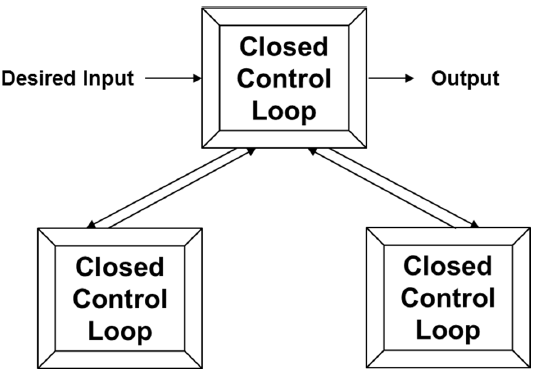
\includegraphics[width=0.4\linewidth]{25-hierachical.png}
    \caption{Hierarchiczna organizacja zamkniętych pętli sterowania. Źródło: \cite{etsieni2024}.}\label{fig:25-hierachical}
\end{figure}

Pętla \textbf{rozproszona} składa się z komponentów działających w różnych lokalizacjach, które komunikują się ze sobą poprzez mechanizmy przesyłania wiadomości. 

\textbf{Adaptacyjność} pętli to dostosowywanie jej parametrów sterowania w czasie rzeczywistym albo na podstawie modelu, który definiuje pożądany efekt, albo używając analizy statystycznej do budowania modelu na podstawie mierzonych danych.

\textbf{Federacją} nazywamy grupę półautonomicznych pętli sterowania, które wykorzystują formalne kontrakty do regulowania wzajemnych interakcji i zachowania. Kontrakty obejmują zasady przyjmowania nowych członków federacji, regulacje dotyczące widoczności i rodzaju informacji jakie mogę być udostępnianie innym członkom federacji. Każda pętla federacji operuje na swoich lokalnych danych. Następnie decyzje podjęte przez każdą z nich są agregowane i publikowane jako wspólna decyzja federacji.

\textbf{Kognitywną} pętla sterowania nazywamy taką, która z pośród dostępnych jej danych jest w stanie wyrozumować nowe dane, informację i finalnie wiedzę, która pomoże jej osiągać cele zarządzania.

\subsubsection{OODA}
Architektura pętli OODA \cite{boyd1995} jest widoczna na Rysunku \ref{fig:25-ooda}.

Widoczne jest iż, każdy element posiada komunikację na trzech płaszczyznach:
\begin{itemize}
    \item Otrzymywanie danych od poprzedniego elementu lub ze środowiska zewnętrznego.
    \item Przekazywanie feedbacku do elementu „Observe” (z wyjątkiem „Orient”).
    \item Przekazywanie danych do następnego elementu lub do środowiska zewnętrznego.
\end{itemize}

Dodatkowo, element „Orient” może przekazywać swoje dane zarówno do „Observe”, jak i do „Act”. Ze środowiskiem zewnętrznym mogą komunikować się jedynie elementy „Observe” oraz „Act”, przy czym każdy z nich realizuje komunikację w innym kierunku. Mimo że pętla OODA może wydawać się sekwencyjna, w rzeczywistości każdy element działa w sposób ciągły, a jego aktywacja (pobudzenie) następuje na zasadzie otrzymania danych.


\begin{figure}[!h]
    \centering 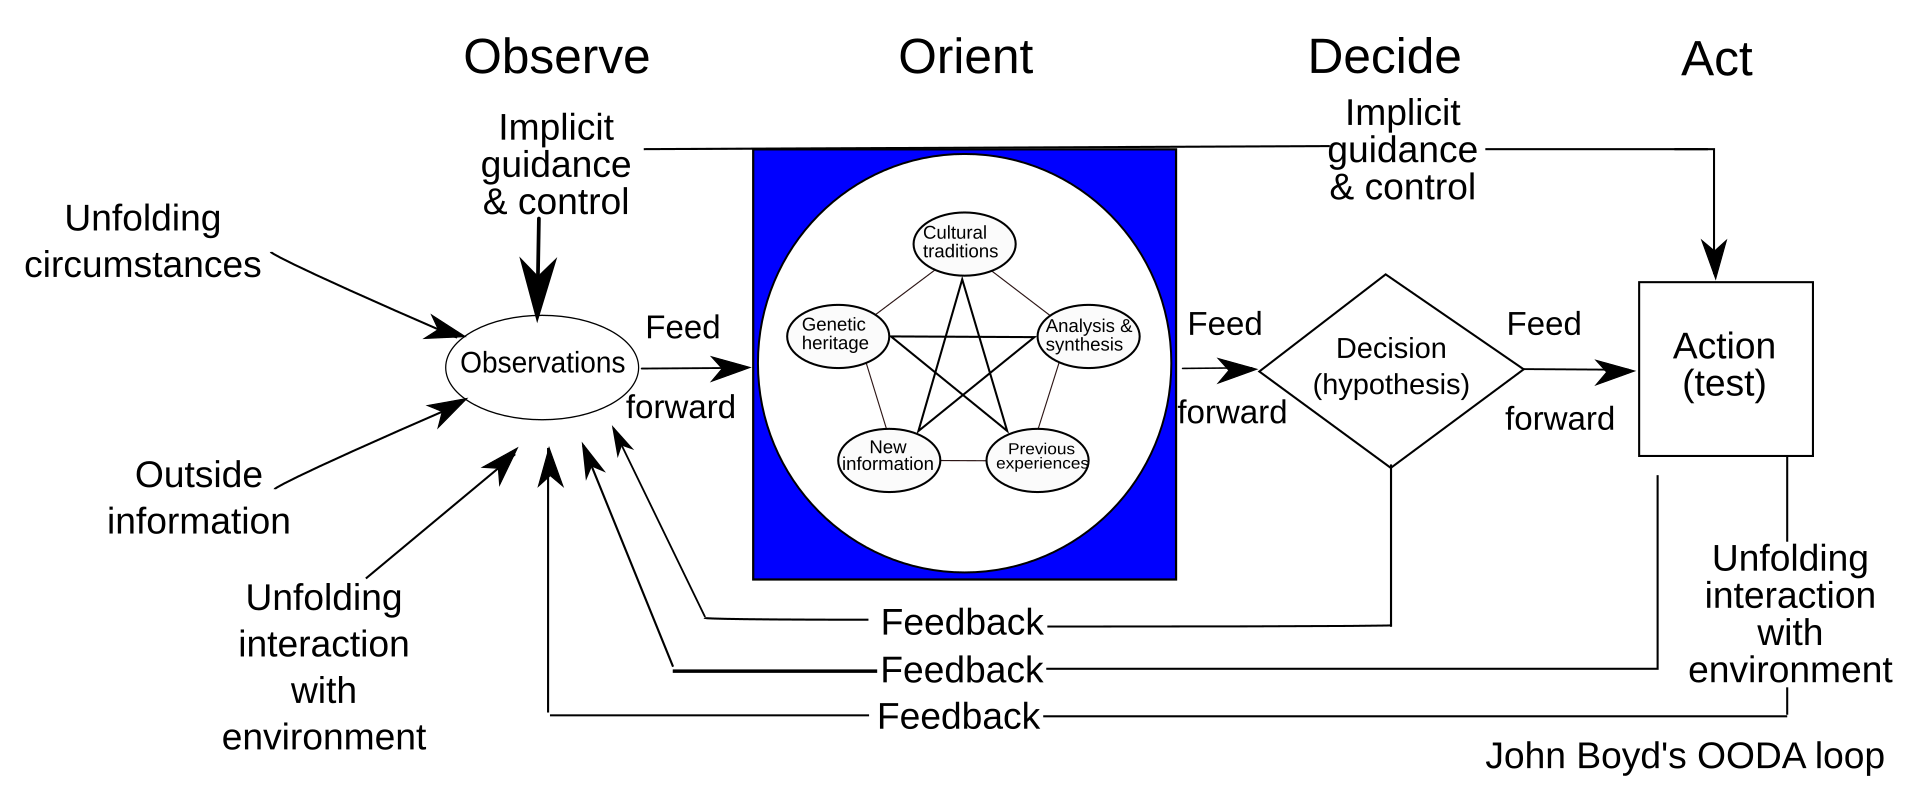
\includegraphics[width=1\linewidth]{25-ooda.png}
    \caption{Architektura pętli OODA. Źródło: \cite{etsieni2024}.}\label{fig:25-ooda}
\end{figure}

\subsubsection{MAPE-K}
Architektura pętli MAPE-K \cite{kephart2003} jest widoczna na Rysunku \ref{fig:25-mapek}.

Jest to pętla sekwencyjna, w której każdy element komunikuje się jedynie na dwóch płaszczyznach:
\begin{itemize}
    \item Otrzymuje dane od poprzedniego elementu (lub ze środowiska zewnętrznego, jeśli jest to moduł „Monitor”).
    \item Przekazuje dane następnemu elementowi (lub do środowiska zewnętrznego, jeśli jest to moduł „Execute”).
\end{itemize}

Dodatkowo, każdy element jest podłączony do „Knowledge”, które pełni funkcję wspólnego repozytorium wiedzy. Generowanie oraz konsumpcja wiedzy stanowią osobny proces komunikacyjny i nie są częścią \hyperlink{def:workflow}{\textit{workflow}} pętli sterowania.

\begin{figure}[!h]
    \centering 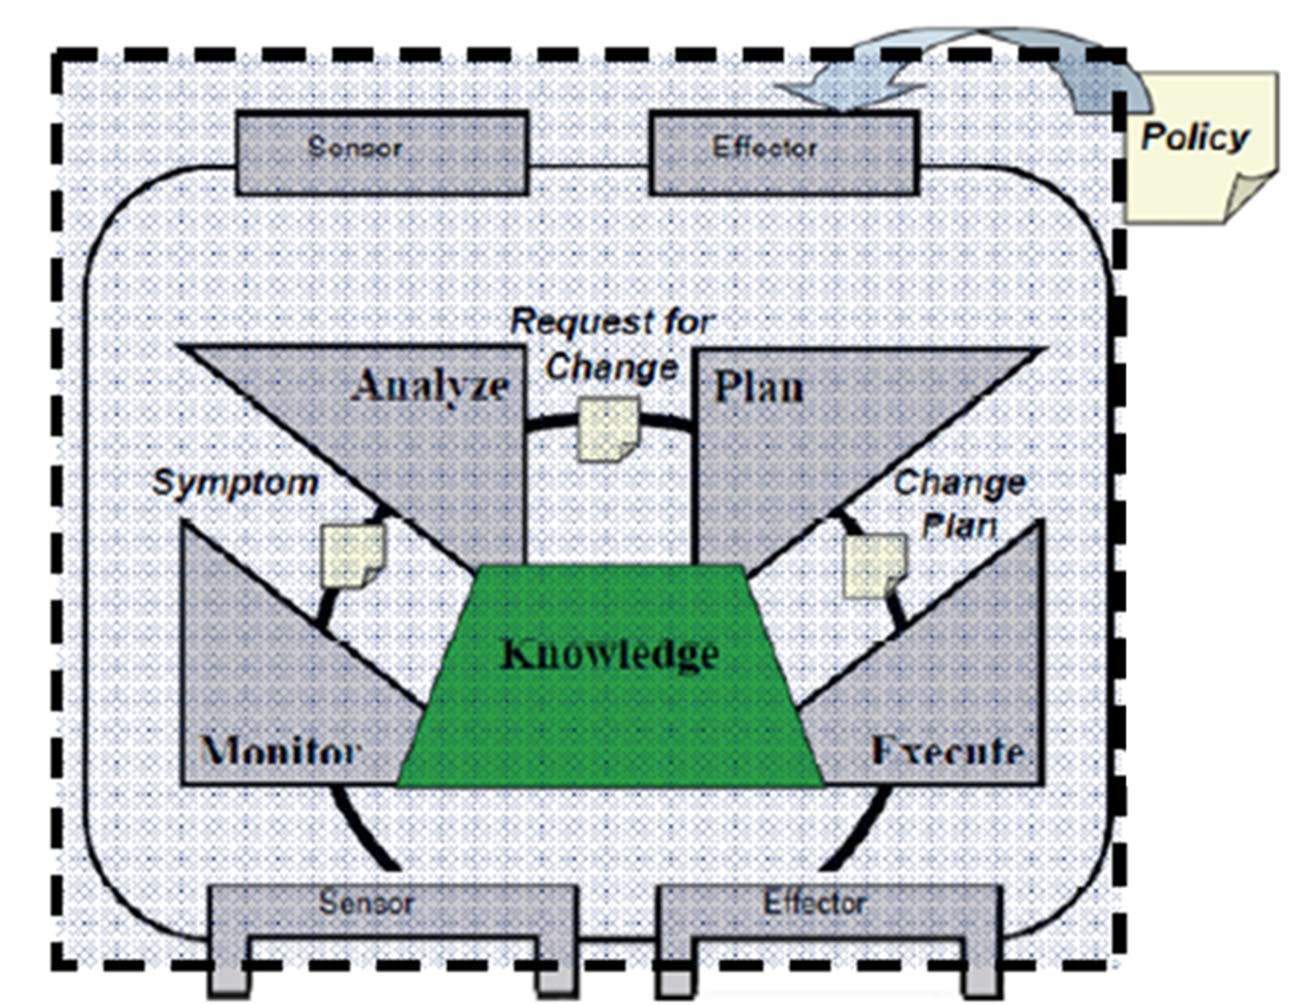
\includegraphics[width=0.5\linewidth]{25-mapek.png}
    \caption{Architektura pętli MAPE-K. Źródło: \cite{etsieni2024}.}\label{fig:25-mapek}
\end{figure}

\subsubsection{Focale}

Architektura pętli Focale \cite{strassner2007} jest przedstawiona na Rysunku \ref{fig:25-focale}. Workflow tej pętli jest sekwencyjne, jednak dzięki wspólnej szynie danych każdy element może komunikować się bezpośrednio z innymi komponentami. Istotnym atrybutem tej szyny jest natywna obsługa modelu informacji DEN-ng \cite{strassner2003} oraz ontologii DENON-ng \cite{strassner2007}. Dodatkowo, każdy element pętli jest połączony z „Autonomic Managerem”, koncepcją zaczerpniętą z \cite{kephart2003}. Pętla Focale może przybierać różne przebiegi w kolejnych iteracjach, w zależności od stanu systemu zarządzanego. Wyróżnia się:
\begin{itemize}
    \item Pętlę utrzymaniową – występuje, gdy system nie wymaga akcji naprawczych ani optymalizacyjnych.
    \item Pętlę rekonfiguracyjną – uruchamianą, gdy stan aktualny systemu różni się od stanu pożądanego, co wymaga podjęcia działań korygujących.
\end{itemize}

\begin{figure}[!h]
    \centering 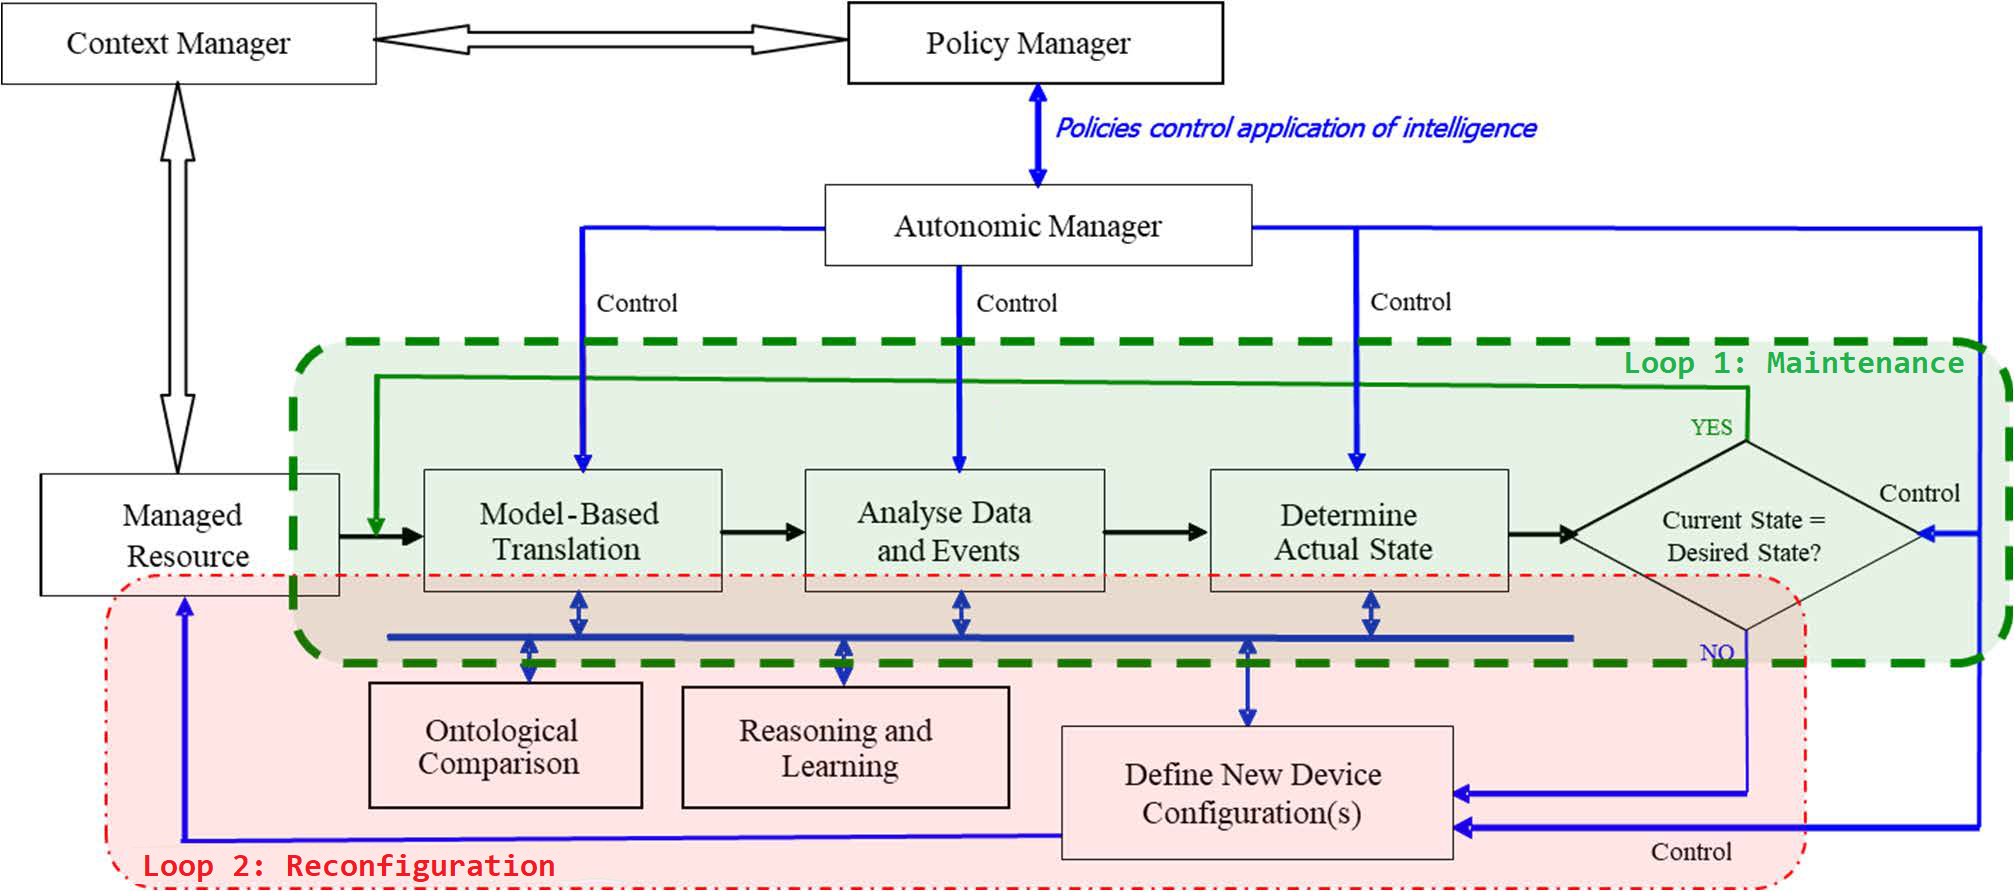
\includegraphics[width=1\linewidth]{25-focale.png}
    \caption{Architektura pętli Focale. Źródło: Opracowanie własne na podstawie \cite{etsieni2024}.}\label{fig:25-focale}
\end{figure}

\subsubsection{GANA}
Architektura GANA (Generic Autonomic Network Architecture) \cite{etsigana2018} jest przedstawiona na Rysunku \ref{fig:25-gana}. Nie definiuje ona pojedynczej pętli sterowania, lecz stanowi zbiór hierarchicznie powiązanych pętli sterowania. Pętle najniższego poziomu implementują tzw. szybkie pętle sterowania, które wykorzystują minimalny poziom kognitywności lub nie stosują jej wcale. W miarę przechodzenia na wyższe poziomy hierarchii, stopień zastosowania mechanizmów kognitywnych wzrasta, co sprawia, że procesy sterowania stają się bardziej złożone, ale również wolniejsze.

\begin{figure}[!h]
    \centering 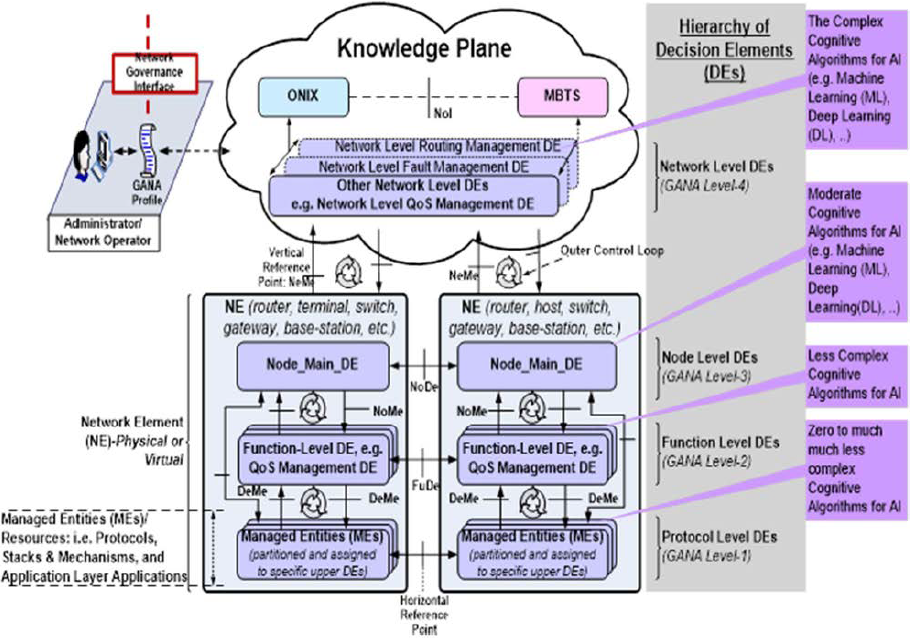
\includegraphics[width=1\linewidth]{25-gana.png}
    \caption{Architektura pętli GANA. Źródło: \cite{etsieni2024}.}\label{fig:25-gana}
\end{figure}

\subsubsection{COMPA}
Architektura COMPA (Control, Orchestration, Management, Policies, Analytics) \cite{doyle2014} jest przedstawiona na Rysunku \ref{fig:25-compa}. Samo workflow pętli nie wnosi istotnych nowości w porównaniu do wcześniej opisanych modeli pętli sterowania. Jednak warto zauważyć, że system zarządzany (automation target) w jednej instancji pętli COMPA może być inną instancją tej samej pętli, co wprowadza rekurencyjną strukturę sterowania.

\begin{figure}[!h]
    \centering 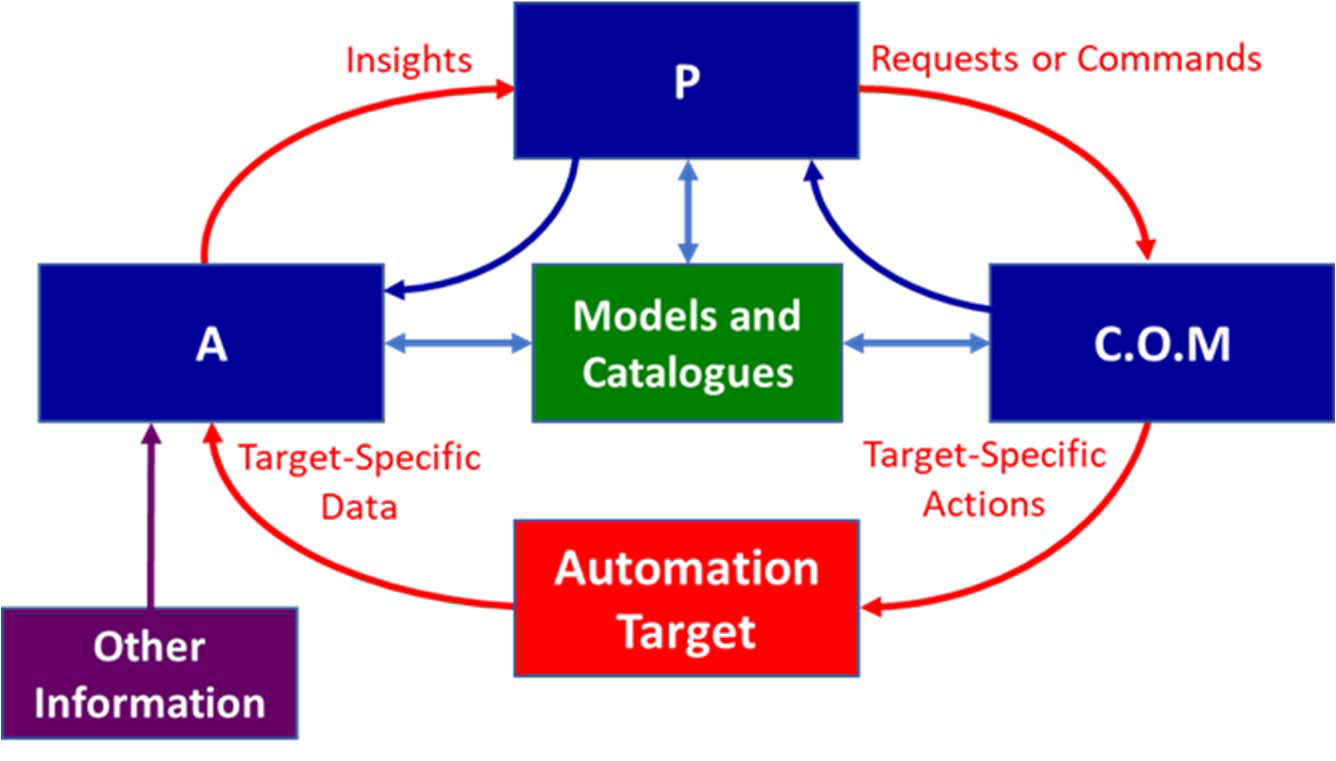
\includegraphics[width=0.5\linewidth]{25-compa.png}
    \caption{Architektura pętli COMPA. Źródło: \cite{etsieni2024}.}\label{fig:25-compa}
\end{figure}

\subsubsection{Focale v3}
Architektura pętli Focale v3 \cite{strassner2009} jest widoczna na Rysunku \ref{fig:25-focalev3}. Jest to kolejna wersja architektury Focale, która to zamiast używać dwóch alternatywnych pętli proponuje dwie nieustannie działające pętle. Jedna zewnętrzna, używana do rekoncyliacji systemu zarządzanego na większą skale w ramach reagowanie na zmiany kontekstu środowiska. Druga wewnętrzna, do rekoncyliacji w ramach jednego określone kontekstu (sytuacji) np. w jednej iteracji. Obie mają 3 alternatywne przebiegi inspirowane \cite{minsky1986}. Przebieg reaktywny używany jest w wypadku gdy zmiany kontekstu już kiedyś się wydarzyły i były przeanalizowane. Przebieg obradujący (ang. \textit{deliberative}) jest wykorzystywany gdy zmiana kontekstu jest znana, ale jej detale nie są jeszcze zrozumiane na tyle, aby móc podjąć natychmiastową akcję. Przebieg refleksyjny ma miejsce, gdy zachodzą zupełnie nowe zmiany kontekstu i system musi się dopiero nauczyć jak sobie z nimi radzić. W kontekście komunikacji elementów wersja ta nie wnosi nic poza to co pętla FOCALE.

\begin{figure}[!h]
    \centering 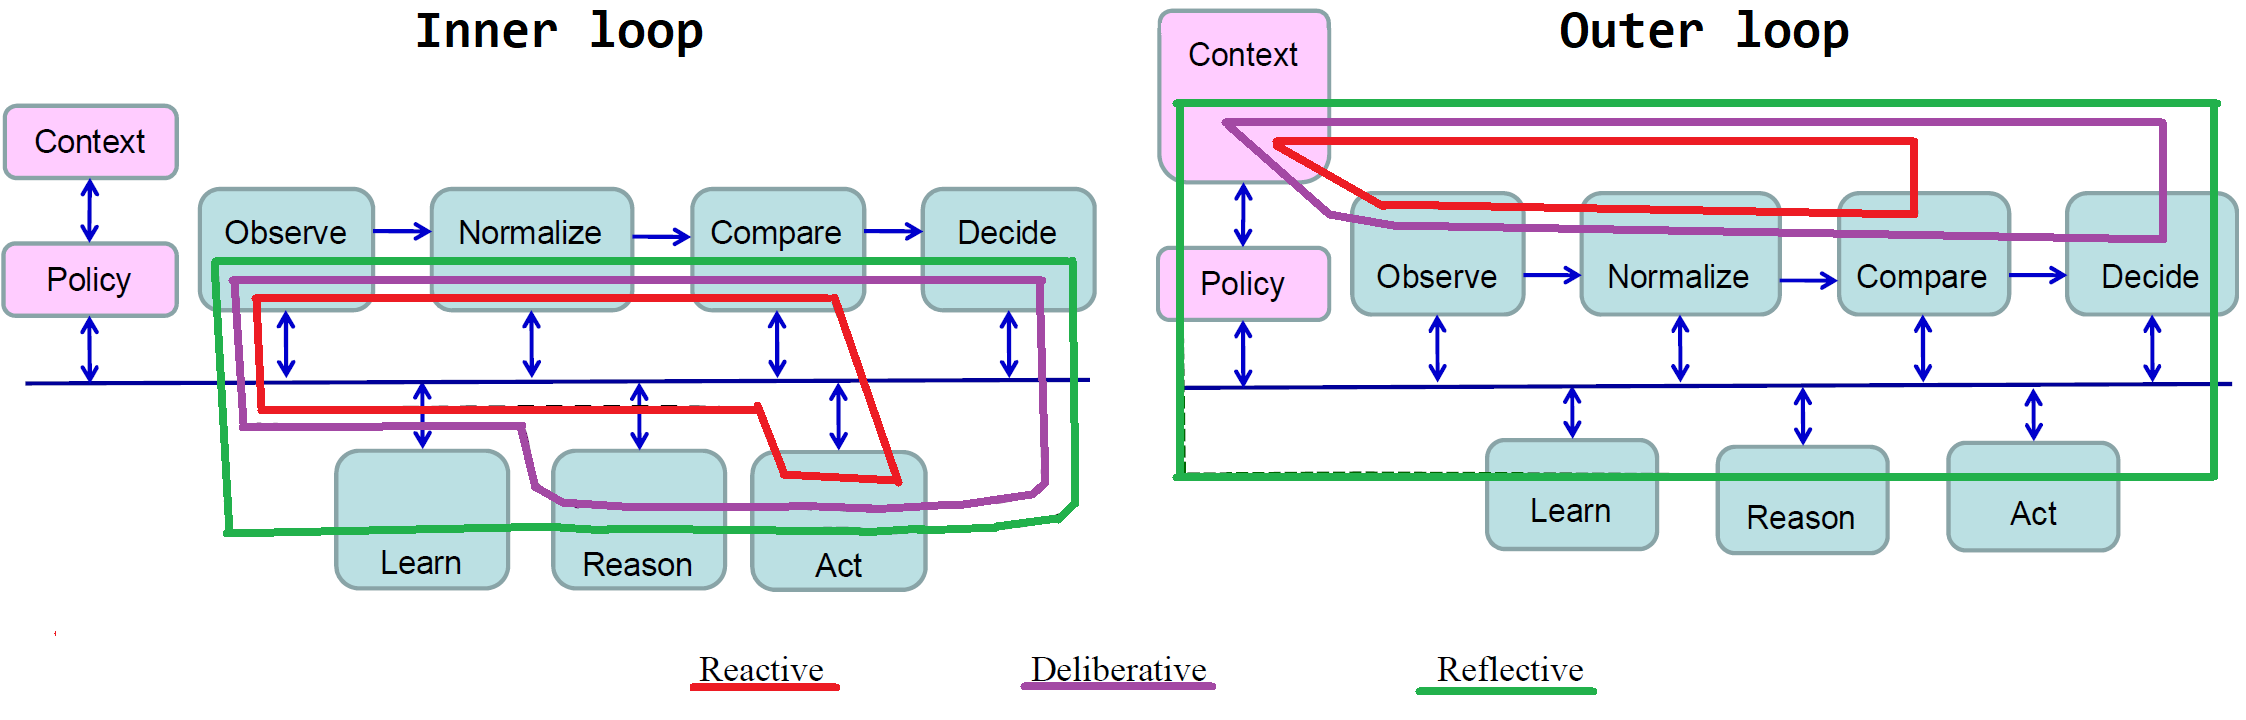
\includegraphics[width=1\linewidth]{25-focalev3.png}
    \caption{Architektura pętli Focale v3. Źródło: Opracowanie własne na podstawie \cite{etsieni2024}.}\label{fig:25-focalev3}
\end{figure}
